
\documentclass[../main.tex]{subfiles}

\begin{document}

Our results demonstrate that under certain circumstances, LeafAI is capable of rivaling the ability of a human programmer in matching patients eligible to clinical trials. Indeed, in numerous cases we found LeafAI and human programmer executing similar queries, such as for Hepatitis C (NCT04852822), Chronic Lymphocytic Leukemia (NCT04852822), Multiple Sclerosis (NCT03621761), and Diabetes Mellitus (NCT03029611), where LeafAI and the human programmer ultimately matched a similar number of patients.

One notable pattern is that LeafAI consistently finds a higher number of potentially eligible patients. As we have not done manual chart review of the patients found, it is difficult to determine the proportion of true positive versus false negative eligible patients compared to eligible patients found by the human programmer. We hypothesize that in many cases, LeafAI's Knowledge Base played a key role both finding additional eligible patients, but also sometimes in unnecessarily excluding otherwise eligible patients. For example, 

% Talk about time spent

\begin{figure}[p]
  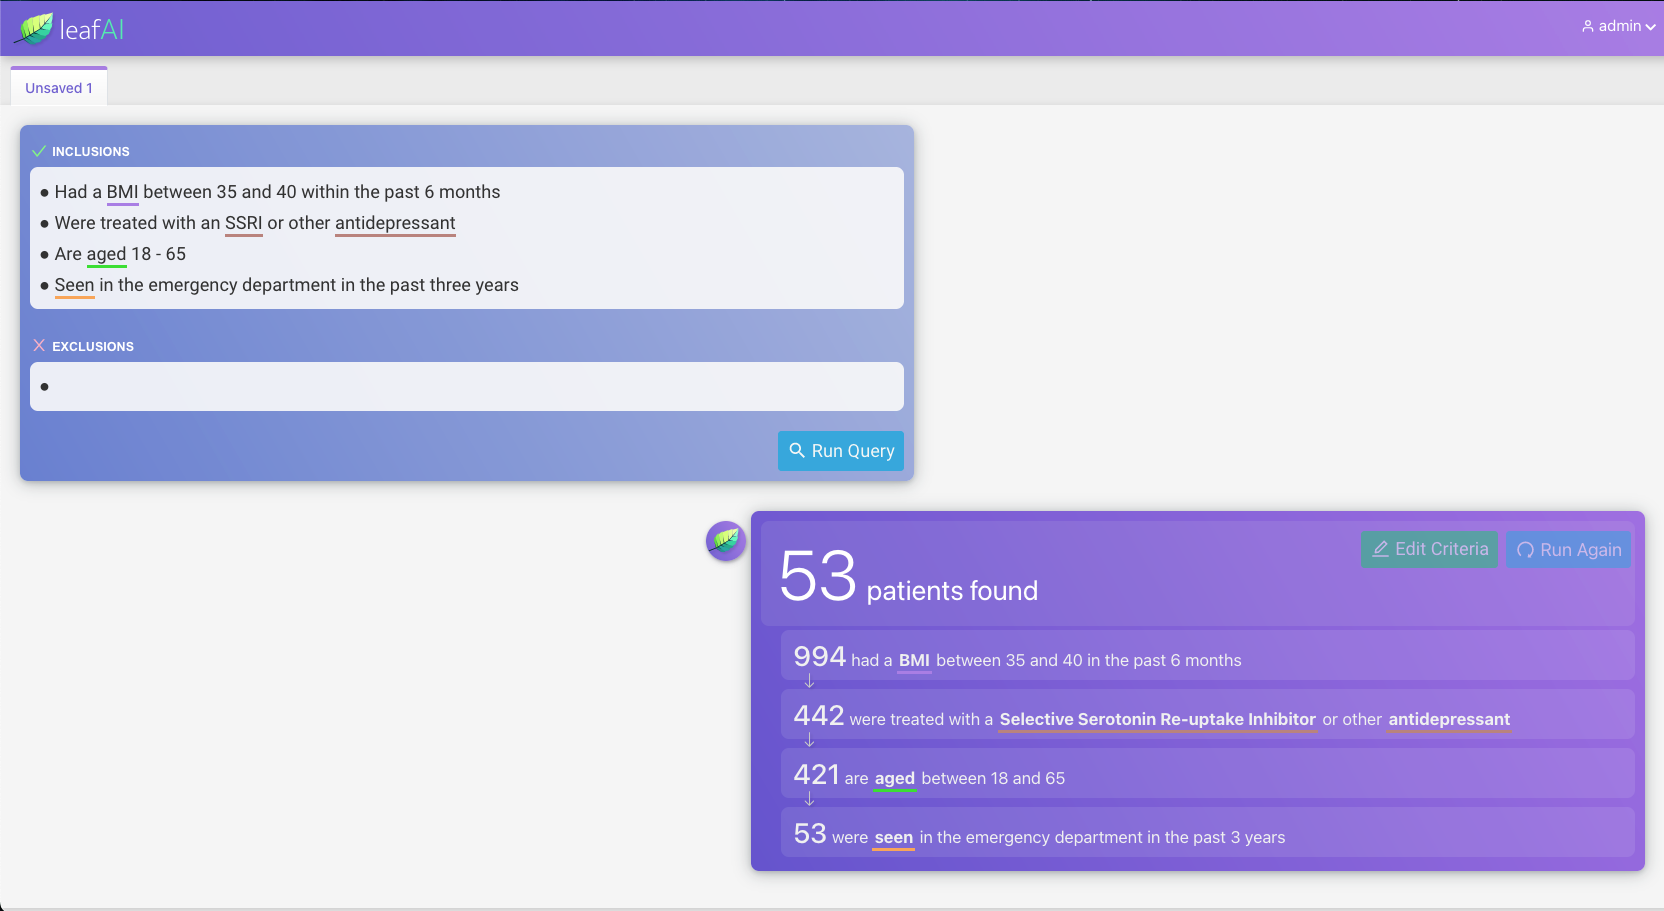
\includegraphics[scale=0.26]{figures/leafai_screenshot.png}  
\caption{Example screenshot of the LeafAI web application, which is currently in development.}
\label{fig_leafai_screenshot}
\end{figure}

\subsection*{Limitations}
\subsection*{Future work}

\end{document}